\documentclass[a4paper, oneside]{book}

%% Language and font encodings
\usepackage[frenchb]{babel}

\usepackage[utf8]{inputenc}
\usepackage[T1]{fontenc}

\usepackage{verbatim}
\usepackage{enumitem}
\usepackage[colorlinks=true, allcolors=blue]{hyperref}

% creation de la commande circled, mot entoure d'un cercle
\newcommand*\circled[1]{\tikz[baseline=(char.base)]{% <---- BEWARE
            \node[shape=circle,draw,inner sep=2pt, color=pumpkin] (char) {#1};}}

% Using \hfuzz allows \hbox to be overfull to the given amount before a warning is raised
\hfuzz = 5pt

% quotes package
\usepackage[autostyle, maxlevel = 2]{csquotes}

% bibliography package            
\usepackage[backend = biber, style = numeric]{biblatex}   
\addbibresource{references.bib}            

% glossary package
\usepackage{nameref}
\usepackage[toc, numberedsection=nameref]{glossaries}

% loading glossary file
\loadglsentries{Glossaire/glossaire.tex} 
\makeglossaries

% package for references and links 
\usepackage{caption}

% package for insertion of pdf pages
\usepackage{pdfpages}

% package to change behavior of floats numbering
\usepackage{chngcntr}
\counterwithout{figure}{chapter}

% pour les images
\usepackage{graphicx}
\usepackage{caption} 
\usepackage{float} 
\usepackage{wrapfig}

%% pour les tableaux
\usepackage{array}
\usepackage{tabularx}
\usepackage{multirow}
\usepackage{slashbox}
\usepackage{colortbl}
\usepackage{framed}
\usepackage{adjustbox}

% pour les maths
\usepackage{amsmath}
\usepackage{amsfonts}
\usepackage{amssymb}
\usepackage{mathrsfs}  
\usepackage{pifont}
\newcommand{\cmark}{\ding{51}}
\newcommand{\xmark}{\ding{55}}

%% package for landscape page view
\usepackage{pdflscape}
\usepackage{rotating}

%% pour dessiner des graphiques et des schemas
\usepackage{tikz}
\usepackage{tkz-graph}
\usetikzlibrary{calc, decorations.pathreplacing}

% Pgfplots
\usepackage{pgfplotstable}
\usepackage{pgfplots}
\usetikzlibrary{pgfplots.groupplots}
\pgfplotsset{compat=1.12}

% définitions des couleurs
\usepackage{color}
  \definecolor{grey}{rgb}{0.4,0.4,0.4}
  \definecolor{blue}{rgb}{0.2,0.3,0.6}
  \definecolor{teal}{rgb}{0.1,0.4,0.4}
  \definecolor{green}{rgb}{0.1,0.7,0.2}
  \definecolor{red}{rgb}{0.8,0.1,0.2}
  \definecolor{pumpkin}{rgb}{0.9, 0.3, 0}

%% Pour l'intégration de code SQL
\usepackage{listings} 
\usepackage{listingsutf8}
\lstloadlanguages{JAVA, SQL}
\lstset{ % affichage du code par défaut
    inputencoding=utf8/latin1,
    basicstyle=\footnotesize\sf,
    morecomment=[s]{/*}{*/},
    morecomment=[l]{//}, 
    keywordstyle=\sffamily\bfseries\color{teal},
    commentstyle=\itshape\color{grey},
    stringstyle=\rmfamily\color{pumpkin},
    tabsize=2, frame=single, breaklines=true,
    showspaces=false, showstringspaces=false,extendedchars=true, 
    numbers=left, numberstyle=\tiny,
    extendedchars=true,
    literate={\$}{{{\$}}}1 {é}{{\'e}}1,    
}

%% definition de style pour une ligne entiere d'un tableau
\newcolumntype{+}{>{\global\let\currentrowstyle\relax}}
\newcolumntype{^}{>{\currentrowstyle}}
\newcommand{\rowstyle}[1]{\gdef\currentrowstyle{#1}%
#1\ignorespaces
}

%% Sets page size and margins
\usepackage[a4paper,top=2cm,bottom=2cm,left=2cm,right=2cm,marginparwidth=1.75cm]{geometry}

%% Pour ecrire des algorithmes
\usepackage[vlined,ruled,linesnumbered]{algorithm2e}

%% Useful packages
\usepackage{amsmath}
\usepackage{amssymb}
\usepackage{amsthm}
\theoremstyle{definition}
\newtheorem{example}{Example}

\usepackage[colorinlistoftodos]{todonotes}

\usepackage{titlesec}
\titleformat{\chapter}[display]{\flushleft\Huge\itshape}{\quad}{0.5em}{}[]
\titleformat{\paragraph}[runin]{\normalfont\normalsize\bfseries}{}{0pt}{}

% leaves out chapter numbers in section numbering
\renewcommand*\thesection{\arabic{section}}

% command defining new chapter type, to be used whith roman page numbering
\newcommand\romanchapter[1]{
  \chapter*{#1}
  \markboth{\MakeUppercase{#1}}{}
  \addcontentsline{toc}{chapter}{#1}
}

\usepackage{fancyhdr}
\setlength{\headheight}{15.2pt}
\pagestyle{fancy}
\rhead{} % empty right header

\begin{document}

\begin{titlepage}
\begin{center}
\begin{sffamily}

{\large
Faculté de Sciences de Montpellier \\[.5cm]
Master 2 AIGLE\\2017 -- 2018\\[2cm]
}


% Title
\rule{\textwidth}{1.6pt}\vspace*{-\baselineskip}\vspace*{2pt} 
\rule{\textwidth}{0.4pt}\\[\baselineskip]
{\LARGE
Notation symbolique de flux de contrôle musicaux et multimédias\\[0.7\baselineskip]
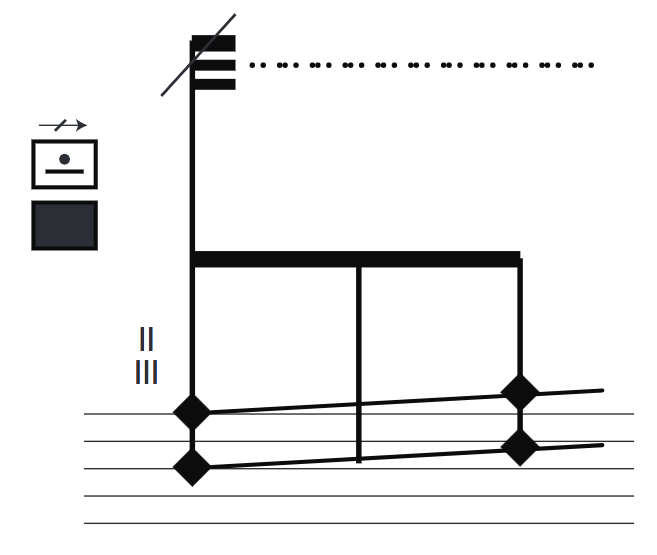
\includegraphics[width=0.3\textwidth]{Paratextes/i/logo.png}
\\[0.5\baselineskip]
Rapport de Stage
}\\[0.2\baselineskip] 
\rule{\textwidth}{0.4pt}\vspace*{-\baselineskip}\vspace{3.2pt}
\rule{\textwidth}{1.6pt}\\[\baselineskip]
\vspace*{2\baselineskip}

% Author and supervisor
\noindent
\begin{center}
     \large
    \emph{\textbf{Étudiant:}}\\
    Vincent Iampietro \\
    \smallskip
    \large
    \emph{\textbf{Encadrant:}}\\
    Jean Bresson\\
    \emph{\textbf{Co-encadrant:}}\\
    Rama Gottfried
\end{center}%



\end{sffamily}
\end{center}
\end{titlepage}

%%%%% PAGE DE GARDE %%%%%
\pagenumbering{Roman}

\setcounter{tocdepth}{1} % profondeur du sommaire, 1 pour sections uniquement

%%%%% SOMMAIRE %%%%%%
\tableofcontents
\clearpage

%%%%% INTRODUCTION %%%%%
\chapter{Introduction}
La notation musicale peut être distinguée en deux approches : une approche prescriptive et une approche descriptive \cite{battier2015}.
La notation prescriptive a pour but de décrire \og comment la musique doit sonner \fg.
Dans cette optique, la partition fait office de référence ou du moins de repère pour l'interprétation d'une pièce. 
La notation descriptive tente de retranscrire \og comment la musique a sonné \fg.
Ainsi, à des fins d'analyse, une pièce peut être caractérisée et fixée sur la \gls{portee}.
Également, la partition est l'outil privilégié du compositeur pour la communication de sa musique, et, au-delà de l'objet fini, constitue un espace de travail.
Pour donner un exemple, la préparation d'une pièce contemporaine par un ensemble musical se fait souvent en collaboration avec le compositeur. La partition constitue alors le support de la discussion et se voit même être modifiée pour les besoins de l'exécution de la pièce. Comme le dit Carmine E. Cella, chercheur et compositeur à l'IRCAM, en parlant de l'écriture musicale : \og le créateur doit s'efforcer de trouver un compromis notationnel entre sa pensée et la réalisation pratique de sa pièce \fg. L'annexe \ref{sec:refletsDeLOmbre} donne deux exemples de partitions représentant la même partie de la pièce \textit{Reflets de l'ombre} (C. E. Cella, 2013), montrant l'adaptation de la notation à des fins d'exécution.

Aussi, procurer des outils aux compositeurs pour leur permettre de noter leurs œuvres est un enjeu primordial. Bien sûr, ces outils ont besoin d'être en phase avec les pratiques de création de leur époque, pour ne pas brider la créativité des utilisateurs.
Or, la musique contemporaine savante et la composition multimédia soulèvent de nouveaux défis d'écriture, en apportant des pratiques inédites, fortement liées à l'usage massif de l'informatique et de l'électronique par les compositeurs. Par conséquent, la présente étude dresse un état de l'art des outils informatiques pour la notation musicale en se posant la question de la pertinence de ces outils pour la transcription des pièces contemporaines.

D'abord, la notation musicale sera décrite sous un axe historique, en s'attardant sur la période  contemporaine et les problématiques notationnelles qu'elle soulève. Ensuite, une vue d'ensemble des moyens informatiques pour la création musicale sera présentée, afin de donner un aperçu au lecteur de l'écosystème actuel dans lequel les compositeurs évoluent et qui influence de fait leurs pratiques. Puis, les outils informatiques existants pour une notation symbolique et traditionnelle de la musique seront détaillés, et leurs caractéristiques seront discutées sous l'angle de la problématique. Enfin, la dernière section s'intéressera aux logiciels et environnements abordant la notation musicale sous un axe contemporain, apportant une dimension interactive aux partitions.

Pour le confort de lecture et la compréhension du rapport, les mots du vocabulaire musical apparaissent en bleu et sont répertoriés dans le glossaire à la fin du document (voir \nameref{main}).




\stepcounter{page}
\pagenumbering{arabic}

%%%%% CHAPTER "FIRST CHAPTER" %%%%%
\chapter{First chapter}
\label{chap:firstChap}
	
\section{First section}
\label{sec:firstScetion}
%\input{OutilsInformatiques/firstSec.tex}	
	
%%%%% CONCLUSION %%%%%
\clearpage
\chapter{Conclusion}
Comme peut en témoigner l'Histoire, la notation musicale n'est pas un processus monolithique. L'écriture de la musique est influencée par le contexte technologique propre à chaque époque. Aussi, la musique contemporaine, qui s'installe à partir des années 50, voit ses pratiques profondément impactées par l'usage de l'électronique et l'informatique. Aujourd'hui encore, l'apparition de nouvelles technologies (machine learning, réalité virtuelle, IoT\footnote{Internet of Things}…) pousse les compositeurs à réinventer leur relation avec la musique et la manière de la noter. Au-delà de la musique contemporaine, la composition multimédia, tirant profit de la profusion des supports technologiques de notre époque (vidéo, audio, capteurs, actionneurs…), cherche encore un système de notation qui lui serait adéquat. Au moment de la rédaction de cette étude, les technologies pour la création musicale sont trop récentes et trop nombreuses pour pouvoir proposer une pratique notationnelle unique. De fait, chaque compositeur a ses propres besoins en termes d'écriture, ce qui devrait pousser les outils informatiques à proposer plus de fonctionnalités permettant l'invention d'une notation par l'utilisateur.

Or, les logiciels actuels de notation musicale ne répondent qu'en partie à la prérogative d'extensibilité ou de renouveau des pratiques d'écriture de la musique, dans le but de s'accorder avec la création contemporaine. Une première catégorie des logiciels existants intègre bien la notation traditionnelle mais ne fournit que peu de moyens pour l'étendre et l'adapter à l'écriture d'œuvres nouvelles. Une deuxième catégorie de logiciels approche la transcription musicale sous l'angle des pièces électroacoustiques et multimédias, en incorporant aux partitions une dimension interactive. Cependant, cette seconde catégorie délaisse quelque peu l'expressivité symbolique au profit de la description temporelle des processus régissant les œuvres.

Dans ce contexte, le développement du logiciel \textit{symbolist} a été initié afin d'adresser le problème du manque d'outils permettant de transcrire symboliquement les œuvres contemporaines \cite{gottfried2018}.
\textit{symbolist} est un éditeur graphique libre où le compositeur peut créer à volonté tous types de symboles et les enregistrer dans une palette. Ce logiciel est destiné à être encapsulé dans les environnements \textit{OpenMusic} et \textit{Max}, et utilise le protocole OSC pour s'interfacer avec l'extérieur.
La poursuite du développement de \textit{symbolist} constitue le cadre du présent stage. Aussi, la génèse et les caractéristiques du logiciel seront explicitées dans le rapport final d'activités.
Dans la continuité de la période d'étude bibliographique, un recueil du besoin sera effectué auprès des compositeurs de musique contemporaine (de l'IRCAM et d'ailleurs), afin de déterminer précisément les attentes des utilisateurs potentiels de \textit{symbolist}.
De plus, une démarche d'analyse et de rétro-ingénierie sera menée sur le logiciel, étant donné son état avancé de développement.
Enfin, une étape d'organisation et de planification des méthodes de travail sera préalable à l'implémentation de nouvelles fonctionnalités.   
 

\stepcounter{page}
\pagenumbering{Roman}

%%%%% BIBLIOGRAPHIE %%%%%
\printbibliography
\addcontentsline{toc}{chapter}{Bibliographie}

%%%%% TABLE DES FIGURES %%%%%
\listoffigures
\addcontentsline{toc}{chapter}{Table des figures}

%%%%% GLOSSAIRE %%%%%
\printglossary[title={Glossaire}, toctitle={Glossaire}]

%%%%% ANNEXES %%%%%
\lhead{} % remove the left part of the header (section name)
\rhead{\textit{ANNEXES}} % set right header
\appendix
\romanchapter{Annexes}
% Pour faire une référence d'une annexe
% (Annexe \ref{sec:nomsection} page~\pageref{sec:nomsection})
\section{Analyse des besoins pour la notation de la musique contemporaine et la composition multimédia}
\label{sec:analyseBesoins}

L'étude bibliographique, amorcée en amont du stage, a permis de dresser un état des lieux des outils pour la notation musicale. Cependant, les besoins réels en termes de notation doivent être recueillis auprès des principaux intéressés: les compositeurs. Aussi, la démarche de recueil tente de répondre à plusieurs questions: Est-il possible de déterminer un noyau commun adressable des besoins de notation des compositeurs? Ou alors, leurs besoins sont-ils spécifiques à chacun d'eux, ce allant dans le sens d'une notation musicale créée et adaptée à chaque compositeur et à chaque pièce \cite{bosseur2005}?

A l'initiative de Jean Bresson, le groupe de travail \textit{notation} a été lancé à l'Ircam. Ce groupe rassemble des chercheurs, des compositeurs ou encore des réalisateurs\footnote{Un réalisateur en informatique musicale travaille de pair avec un compositeur de musique contemporaine, pour réaliser techniquement les pièces musicales imaginées par le compositeur.} en informatique musicale. Le groupe de travail s'organise autour de discussions, de débats ou de présentations sur le sujet de la notation musicale en musique contemporaine. Aussi, c'est lors de ces séances que l'idée de la création d'un questionnaire pour le recueil des besoins des compositeurs a émergée.
Le questionnaire établi comporte trois questions à réponse ouverte; il a été rendu au plus court dans le but de recevoir le plus de réponses possibles. Les trois questions sont les suivantes
\begin{enumerate}[label={(\arabic*)}]
	\item \textit{Pouvez-vous décrire votre workflow de notation?}: quelles sont les pratiques notationnelles des compositeurs, et les outils qu'ils utilisent.
	\item \textit{Pouvez-vous nommer trois fonctionnalités que vous jugez primordiales dans un logiciel de notation musicale?}: isolement de préoccupations principales des compositeurs en termes de notation.
	\item \textit{Concernant les outils de notation que vous utilisez, y a-t-il des problèmes que vous voudriez adresser?}: problématiques rencontrées par les compositeurs, et leur sentiment général par rapport à leurs outils.  
\end{enumerate}

Le questionnaire a été envoyé à plus de trois cents compositeurs par mail, en tirant profit des listes de diffusion de l'Ircam.
Quinze compositeurs ont répondu, ce qui permet déjà d'analyser et de tirer des motifs de leurs retours. Les résultats pour chaque question sont présentées et analysées ci-après.

\paragraph{Pouvez-vous décrire votre workflow de notation?} Cette première question visait à déterminer quels outils de notation sont utilisés par les compositeurs et dans quelles proportions. Le tableau \ref{tab:workflowNotation} présente tous les types d'outils de notation cités dans les réponses, et pour chacun d'eux le nombre de compositeurs en faisant usage sur les quinze ayant répondu.

\newcolumntype{C}{>{\centering\arraybackslash} X}
\begin{table}[H]
	
    \renewcommand{\arraystretch}{1.5}
    \centering
    
	\begin{tabularx}{\textwidth}{|C|C|C|C|C|}
	\hline
    Papier & Logiciels orientés CWMN & Logiciels orientés électroacoustiques & Logiciels de design graphique (\textit{Adobe Illustrator}, \textit{INKScape}) & Logiciels mixtes (\textit{INScore}) \\
    \hline
    10/15 & 11/15 & 5/15 & 3/15 & 1/15 \\
    \hline
	\end{tabularx}
	
   	\caption{Sondage sur l'utilisation des outils de notation musicale}
    \label{tab:workflowNotation}
	\small
	\textit{Il est a noté que le nombre d'outils utilisés par chaque compositeur variant, le nombre total de réponses n'est pas égal à quinze.}
\end{table}

Les résultats du tableau \ref{tab:workflowNotation} montre que le papier et les logiciels de notation utilisant le système traditionnel occidental sont les plus utilisés par les compositeurs. En effet, le support papier est souvent utilisé par les compositeurs au début de leur phase de composition, pour ne pas brider leur créativité en s'imposant le canevas d'un logiciel. De même, la forte utilisation des programmes de notation orientés CWMN (\textit{Sibelius}, \textit{Finale}, \textit{MuseScore}, etc.) s'explique par la grande diffusion de ces outils sur le marché international, alors que les outils pour la notation de l'électroacoustique relève d'une utilisation plus discrète, touchant en majorité les milieux de la recherche en informatique musicale.
Également à noter, quelques compositeurs (trois parmi quinze) décrivent les stations audionumériques qu'ils utilisent comme de véritables outils de notation de la musique; cela amène à reconsidérer le statut de ces logiciels (voir la discussion de la section \ref{sec:notationMusiqueContemporaine}).

\paragraph{Pouvez-vous nommer trois fonctionnalités que vous jugez primordiales dans un logiciel de notation musicale?} La deuxième question avait pour but de profiler un noyau de caractéristiques dont l'absence dans un outil de notation serait rédhibitoire pour la communauté des compositeurs de musique contemporaine.
Voici la liste des propositions faites par les compositeurs, dans l'ordre de la plus citée à la moins citée:
\begin{itemize}[label=--]
	\item Liberté (flexibilité) dans la composition graphique des partitions (7/11)
	\item Automatisation du rendu graphique (alignement, mise en page…) (6/11)
	\item Rendu audio de la partition (6/11)
	\item Intégration de la CWMN (4/11)
	\item Interopérabilité (4/11)
	\item Visualisation de formes d'ondes, et spectres (3/11)
	\item Symboles de spatialisation (1/11)
\end{itemize}

Seuls onze compositeurs ont bien répondu à cette question, ce qui explique le changement de mesure. Les résultats montrent l'intérêt des compositeurs quant à la liberté d'expression graphique procurée par les logiciels de notation. La qualité de rendu graphique des partitions et l'aisance d'utilisation d'un logiciel est également un impératif. Aussi, les compositeurs réclament une logique de mise en page efficace, pour traiter, par exemple, l'alignement ou l'espacement des éléments graphiques entre eux.
Il est à noter que l'intégration des symboles du système traditionnel occidental n'est pas considéré comme primordial. D'ailleurs, la capacité de connecter un logiciel de notation musicale à d'autres systèmes de production sonore est une considération de même niveau pour les compositeurs. L'impératif d'interopérabilité est liée à l'impératif de rendu audio de la partition (le rendu effectué par les logiciels de synthèse sonore).

\paragraph{Concernant les outils de notation que vous utilisez, y a-t-il des problèmes que vous voudriez adresser?} La dernière question a été formulée pour identifier les faiblesses des outils de notation ou les difficultés qu'ils induisent dans le processus de composition.  Les problèmes identifiés sont les suivants:
\begin{itemize}[label=--]
	\item Mauvais alignement des éléments évoluant à des temporalités différents: par exemple, alignement des éléments de deux portées ayant des signatures rythmiques différentes.
	\item Mauvais alignement des éléments relevant de paradigmes différents: par exemple, alignement d'une forme d'ondes et de notes de musique.
	\item Peu de liberté pour la composition et le dessin graphique.
	\item Pas de vues multiples d'une même partition dans un même logiciel de notation. Le compositeur est alors obligé de répliquer sa partition dans plusieurs logiciels, chacun lui offrant une vue précise de sa partition.
\end{itemize}

La plupart des plaintes recueillies concernent la capacité d'expression et le rendu graphique des logiciels; cela va de pair avec la considération de ces fonctionnalités comme étant primordiales pour un programme de notation musicale.
\clearpage

% Appendix declaration with a 90° rotated figure
\rotatebox{90}{
	\begin{minipage}{0.90\textheight}
		\section{Modèle de l'application symbolist}
		\label{sec:symbolistModelClassDiagram}
		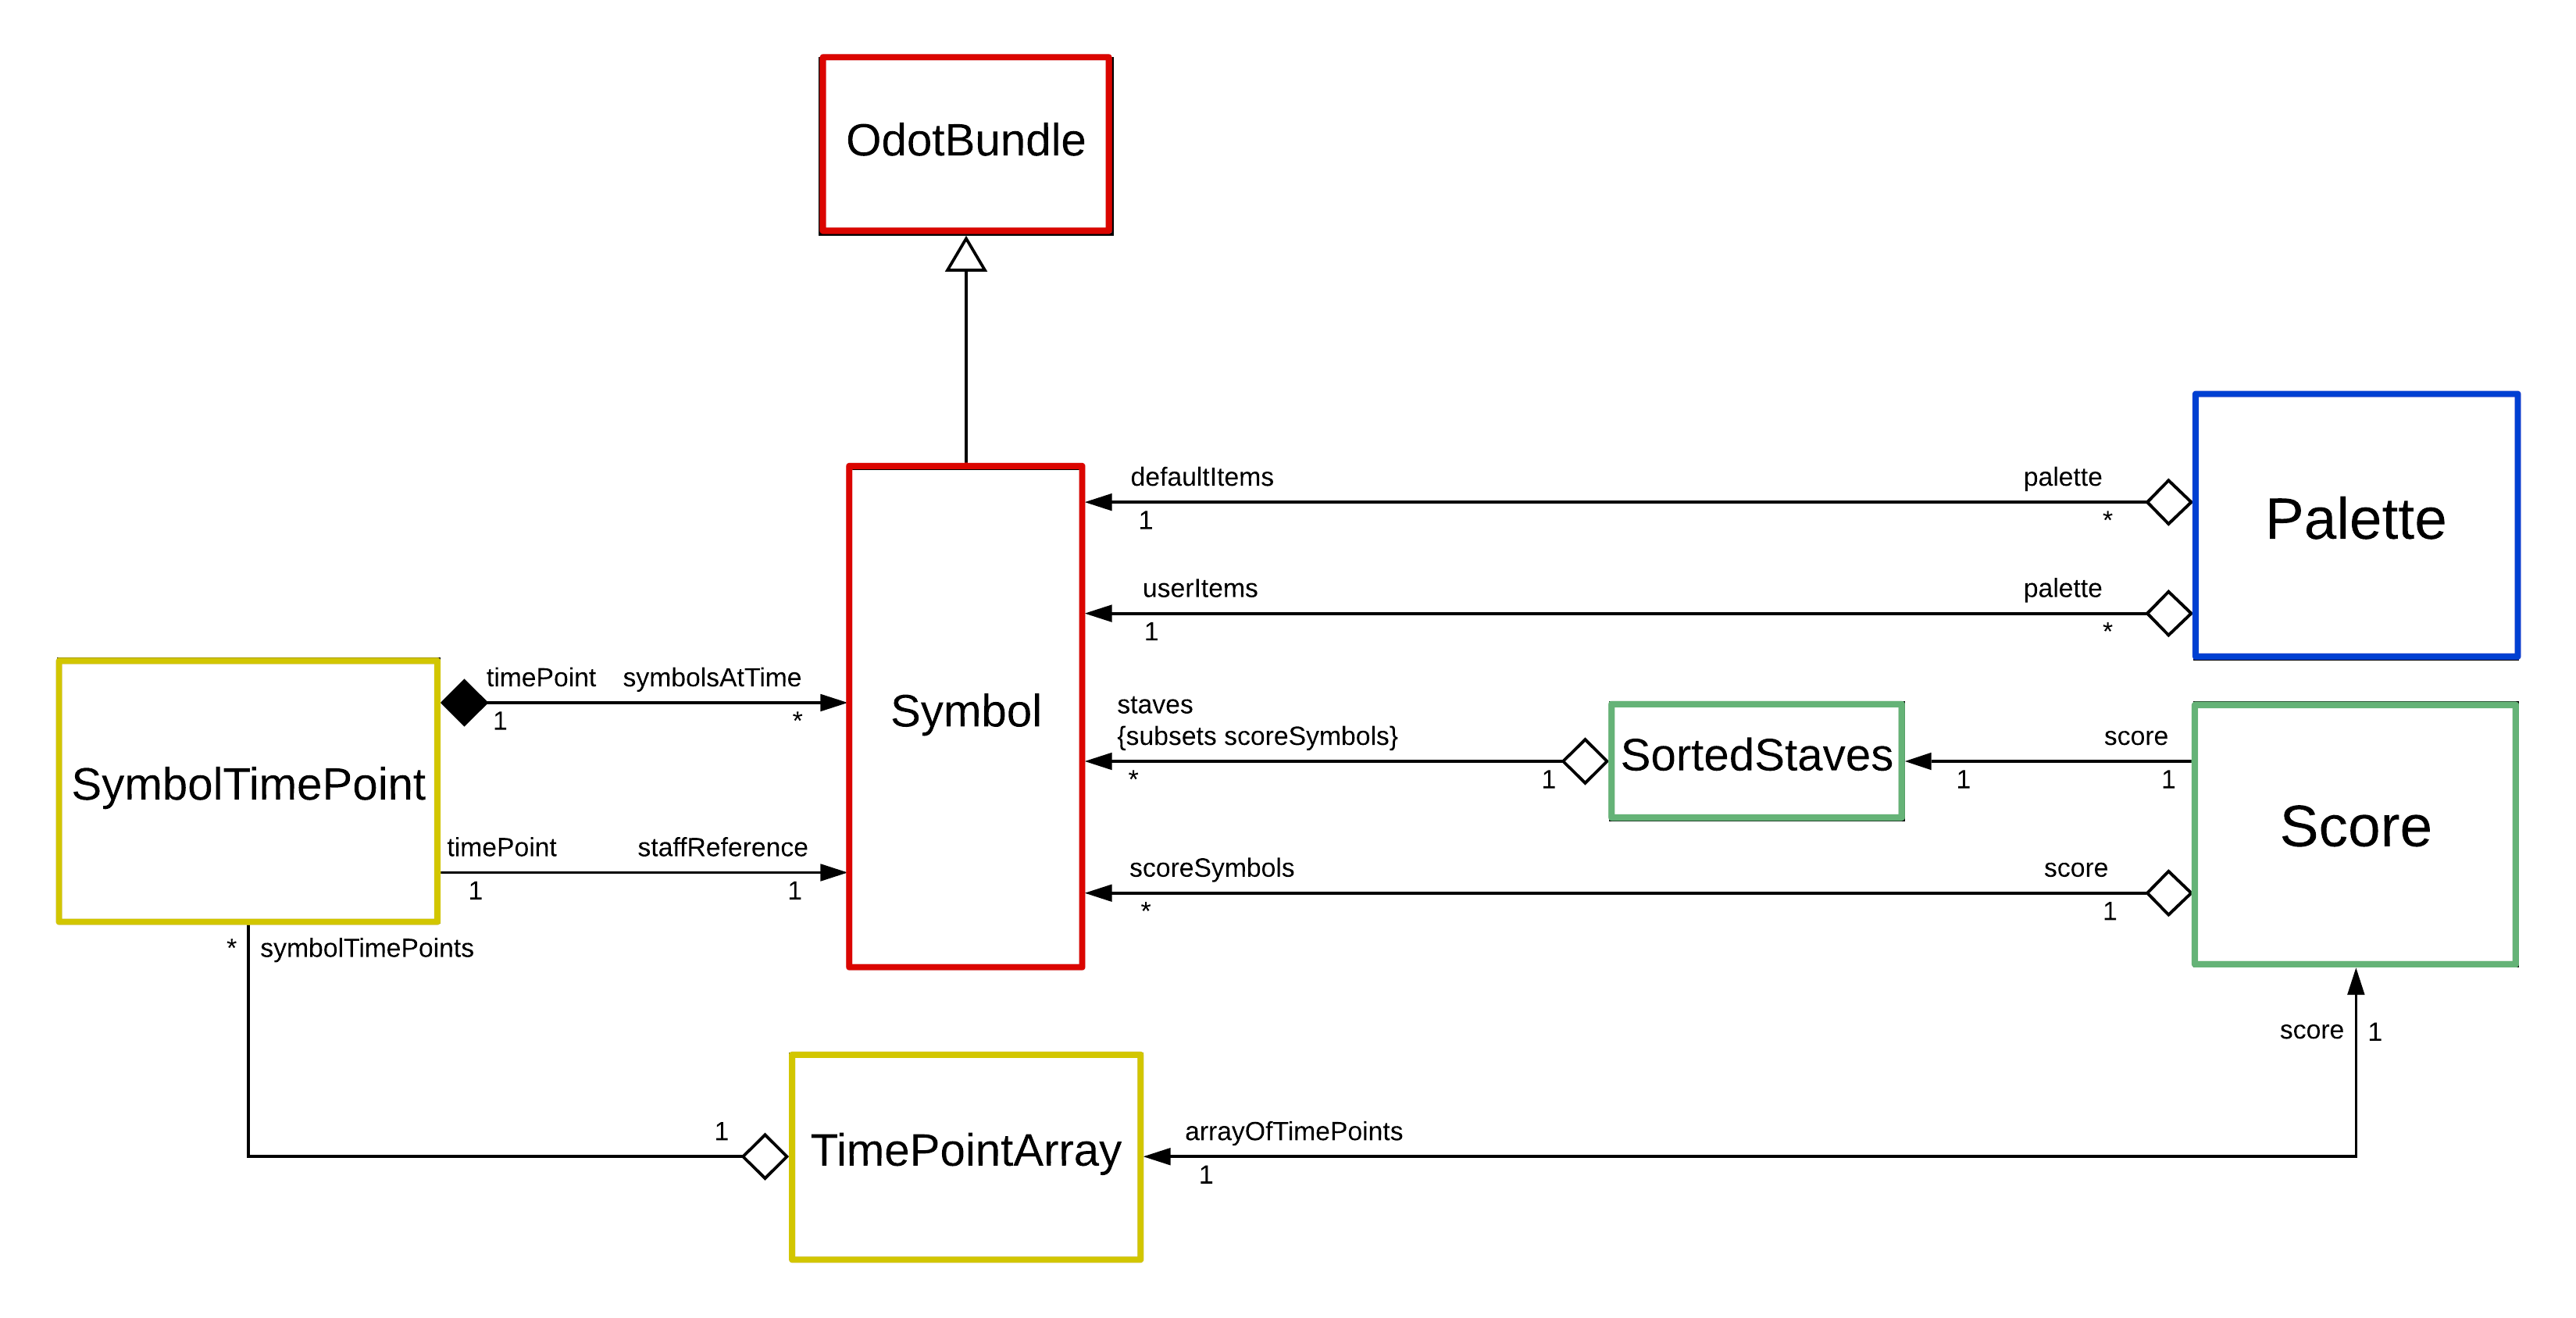
\includegraphics[keepaspectratio=true, width=\textwidth]{Annexes/i/symbolistModelClassDiagram.png}
		\captionof{figure}{Diagramme de classes pour le modèle de l'application symbolist}
		\label{fig:symbolistModelClassDiagram}	
		\medskip
		\small
		\it
		En \textcolor{red}{rouge}, la classe \emph{OdotBundle}, qui encapsule la structure d'un bundle \emph{OSC}, et la classe \emph{Symbol} dont les instances représentent les symboles de la partition. Chaque symbole de la partition possède une structure de bundle OSC, d'où la relation d'héritage entre la classe \emph{OdotBundle} et \emph{Symbol}.
		En \textcolor{blue}{bleu}, la classe \emph{Palette}, regroupant les symboles pouvant être dessinés sur la partition, qu'ils aient été définis par l'utilisateur ou existaient par défaut dans l'application.
		En \textcolor{green}{vert}, les classes \emph{Score} et \emph{SortedStaves} décrivant les symboles présent dans la partition.
		En \textcolor{yellow}{jaune}, les classes \emph{SymbolTimePoint} et \emph{TimePointArray} définissant la logique d'ordonnancement temporel des symboles associés à un \emph{staff}.  
	\end{minipage}
}
\clearpage

\rotatebox{90}{
	\begin{minipage}{0.85\textheight}
		\section{Architecture finale de l'application symbolist}
		\label{sec:symbolistFinalStructure}
		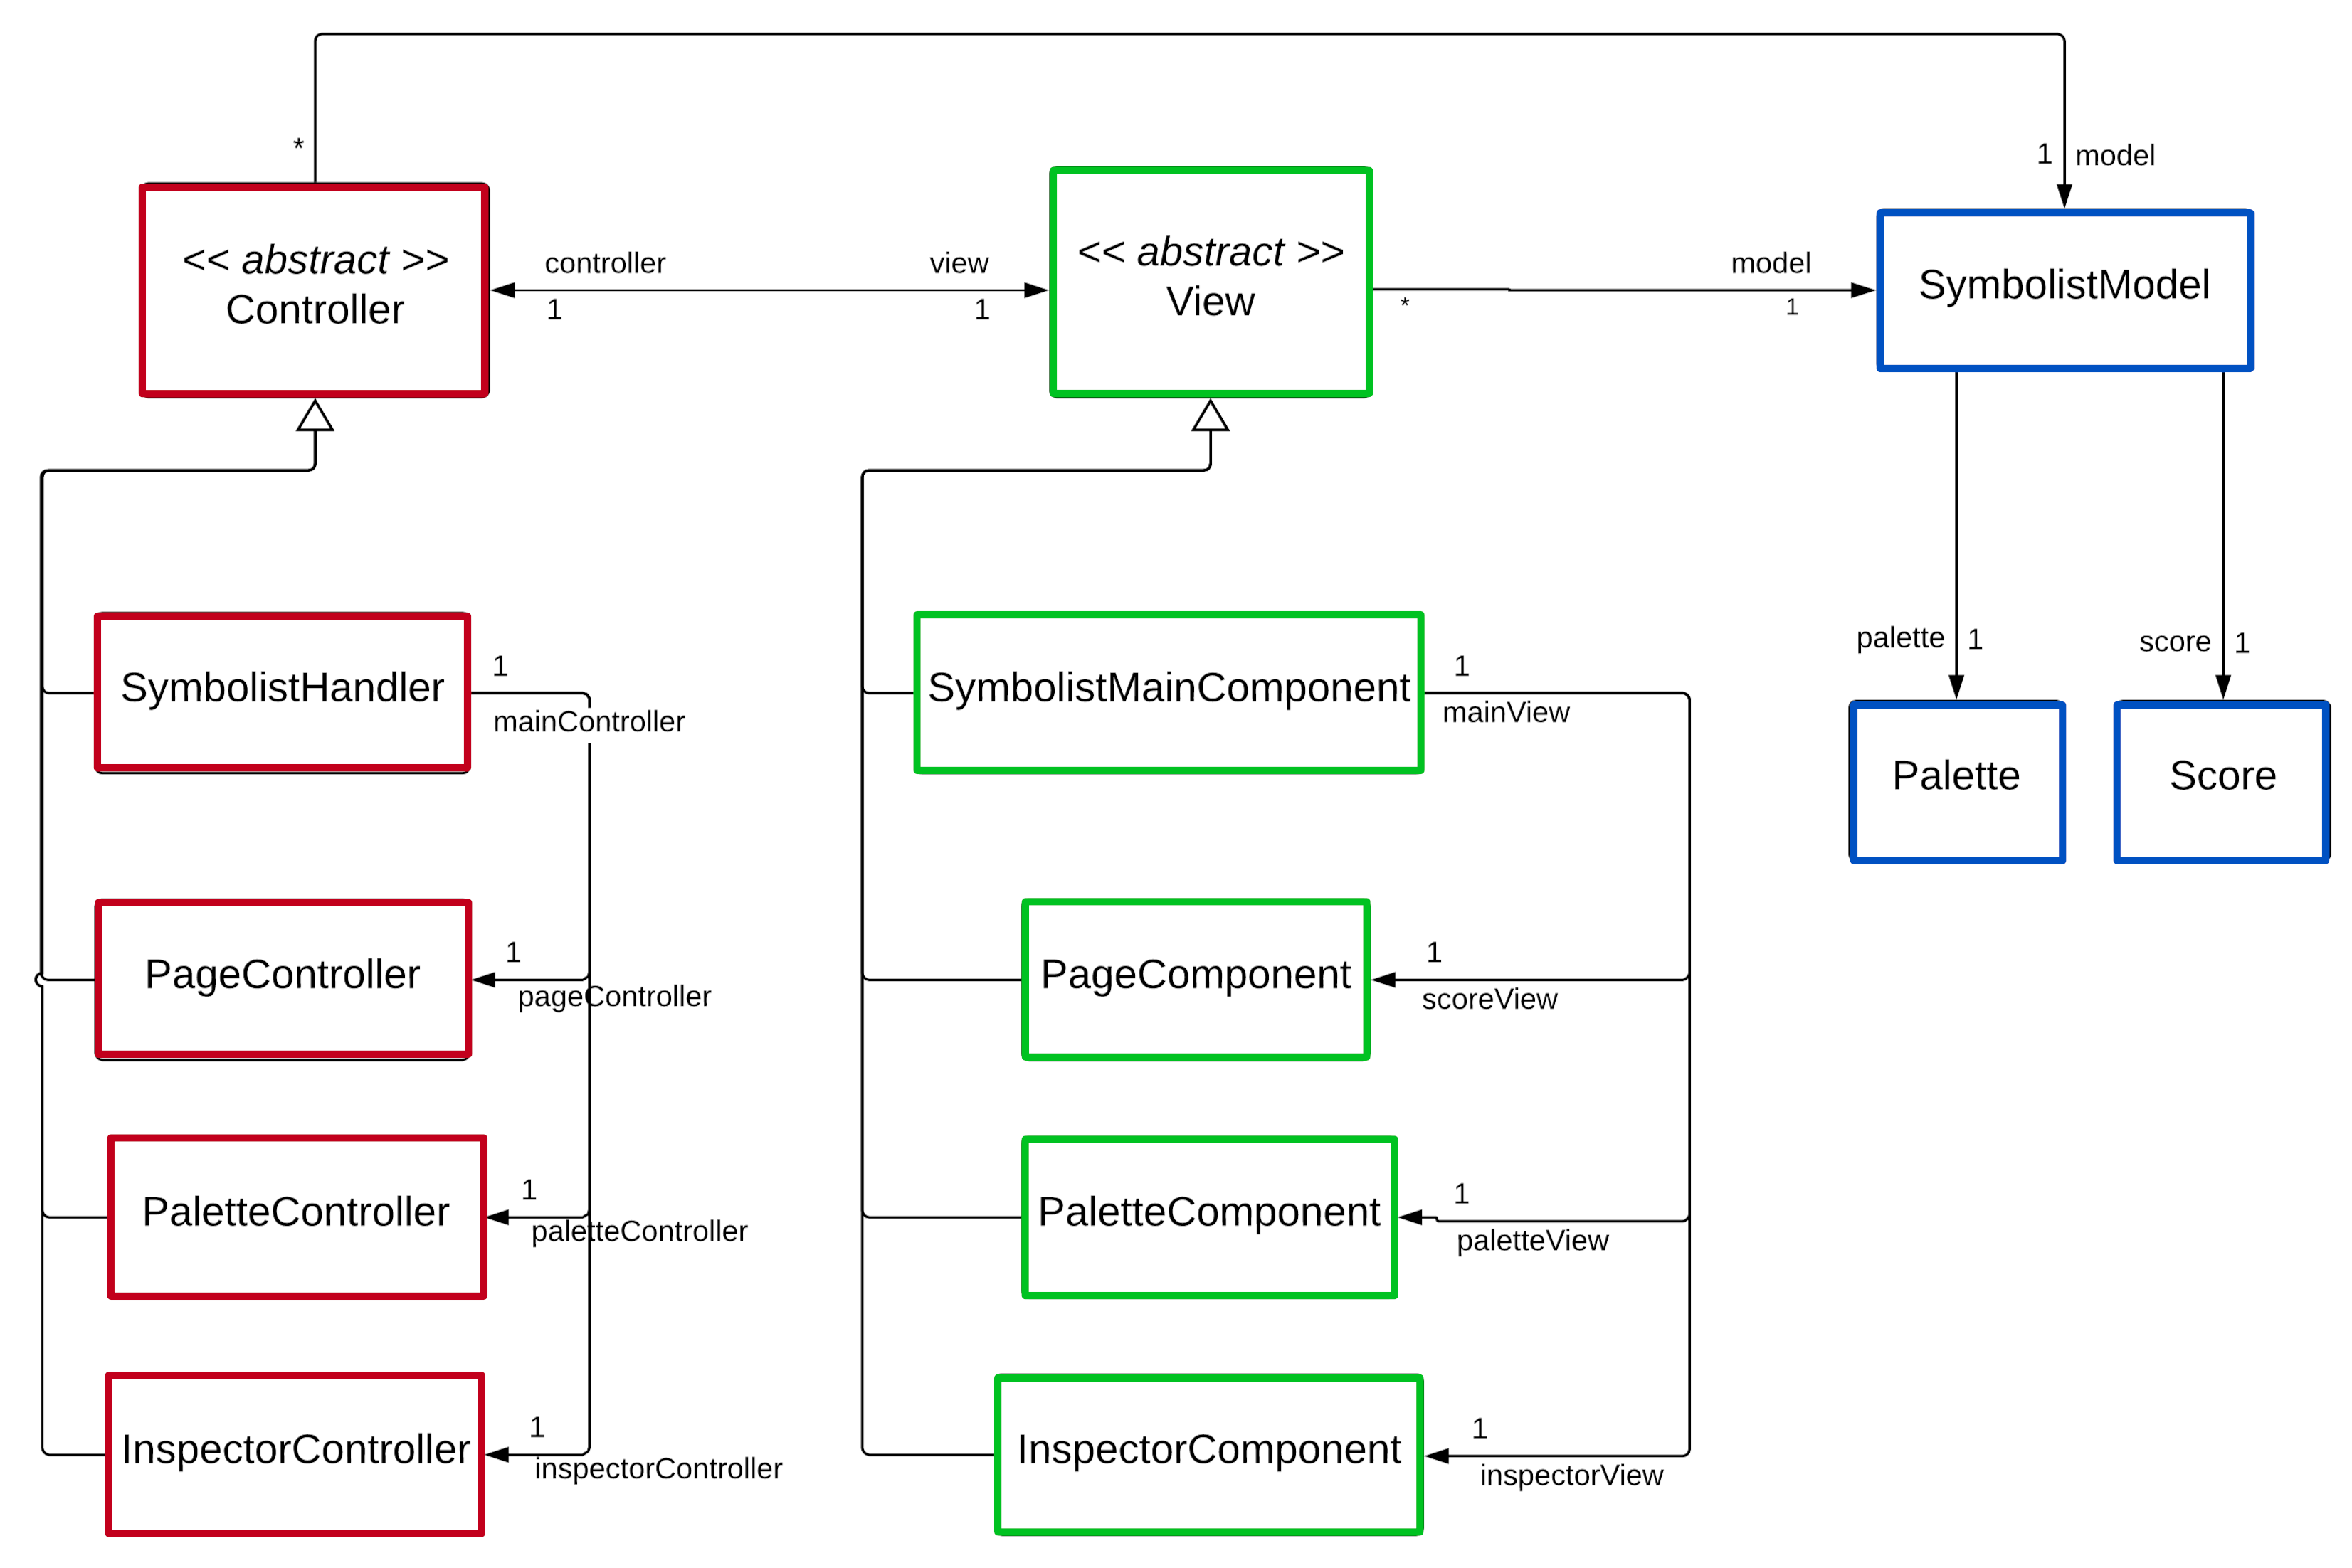
\includegraphics[keepaspectratio=true, width=\textwidth]{Annexes/i/symbolistFinalStructure.png}
		\captionof{figure}{Diagramme de classes présentant l'architecture de l'application symbolist après restructuration}
		\label{fig:symbolistFinalStructure}	
		\medskip
		\small
		\it
		En \textcolor{red}{rouge}, .
		En \textcolor{blue}{bleu}, .
		En \textcolor{green}{vert}, .  
	\end{minipage}
}
\clearpage


\end{document}
